\ihead{Tagesberichte}
\section{Tagesberichte}
\label{sec:tagesbericht}

\begin{itshape}
Information für den Lesenden: Die Angaben zu Beginn und Ende der Arbeitstage schließen eine Mittagspause von durchschnittlich 45min ein.
\end{itshape}

\subsection{Februar}
\subsubsection*{1. Februar - 9:00 bis 16:00 Uhr}
Der erste Arbeitstag begann damit, dass ich freundlich von meinem Betreuer, dem operativen Geschäftsführer Dipl.-Ing. Stefan Wambacher, in Empfang genommen wurde. Nachdem ich mich allen Kollegen, die an diesem Tag anwesend waren, vorgestellt habe, wurde ich von meinem Betreuer in die Grundzüge der Betriebsinternen Problemstellung, welche ich in den drei Monaten des Praktikums lösen soll, eingeführt.

Nachdem sich mein Arbeitsnotebook noch in der Postzustellung befunden hatte, war ich am ersten Tag in meiner Tätigkeit insoweit eingeschränkt, als ich keinen Zugang zu den firmeninternen Systemen hatte. Jedoch brachte ich an meinem ersten Arbeitstag mein eigenes Notebook mit, wodurch ich auf diesem mit dem Rechercheprozess zu Microsoft Dynamics 365 Project Operations beginnen konnte.

Zu besonderen Anlässen - und dieser Tag scheint einer davon gewesen zu sein - setzt sich das anwesende Team zusammen und bekommt von dem Unternehmen ein Mittagessen spendiert. Hierbei konnte ich ersten freundlichen Kontakt mit meinen neuen Kollegen schließen und über deren Aufgabenbereiche erfahren.

\subsubsection*{2. Februar - 9:00 bis 16:45 Uhr}
An meinem zweiten Arbeitstag bekam ich mein fertig eingerichtetes Arbeitsnotebook ausgehändigt, auf dem ich direkt im Anschluss mit einem weiteren neuen Kollegen, Carlos Algarra, virtuell über MS Teams in Kontakt treten durfte. In diesem Meeting wurde mir der Status-Quo der aktuellen Arbeitsverteilung in dem Unternehmen geschildert, sowie die Ergebnisse eines ersten Brainstormings bezüglich der Funktionalitäten des zukünftigen Systems dargelegt.

Nach diesem Meeting habe ich begonnen, auf der Whiteboard-Kollaborationsplattform \href{https://miro.com/de/}{Miro} erste Entitäten in einem Entity-Relation Schema zu entwerfen, auf denen die zukünftigen Prozesse des neuen Systems aufbauen sollen.

\subsubsection*{3. Februar - 9:00 bis 15:10 Uhr}
Zu Beginn des nächsten Tages habe ich die Gestaltung des ER-Schemas fortgesetzt, wobei ich anschließend bei einem erneuten virtuellen Meeting mit Carlos Empfehlungen bezüglich der Verbesserung und des Streamlining meines bisherigen Ansatzes bekommen habe. Hier wurden auch direkt Fragen beantwortet, die bei der Erstellung des Modells aufgekommen sind. Nachdem das gegebene Feedback implementiert wurde, habe ich final überprüft, ob alle Anforderungen, welche bis dato an den Entwurf gestellt wurden, abgedeckt sind und anschließend eine Dokumentation über die wichtigsten Entitäten des Schemas erstellt, um die Nachvollziehbarkeit des Entwurfs sicherzustellen. 

\subsubsection*{6. Februar - 9:00 bis 15:15 Uhr}
Nachdem der letzte Tag mit der Finalisierung des ER-Schemas geendet hatte, wurde dieser Arbeitstag vollends der Prozessgestaltung gewidmet, wobei darauf geachtet wurde, dass alle modellierten Prozesse auch lückenlos an die Entitäten ansetzen. 

\begin{figure}[h]
    \centering
    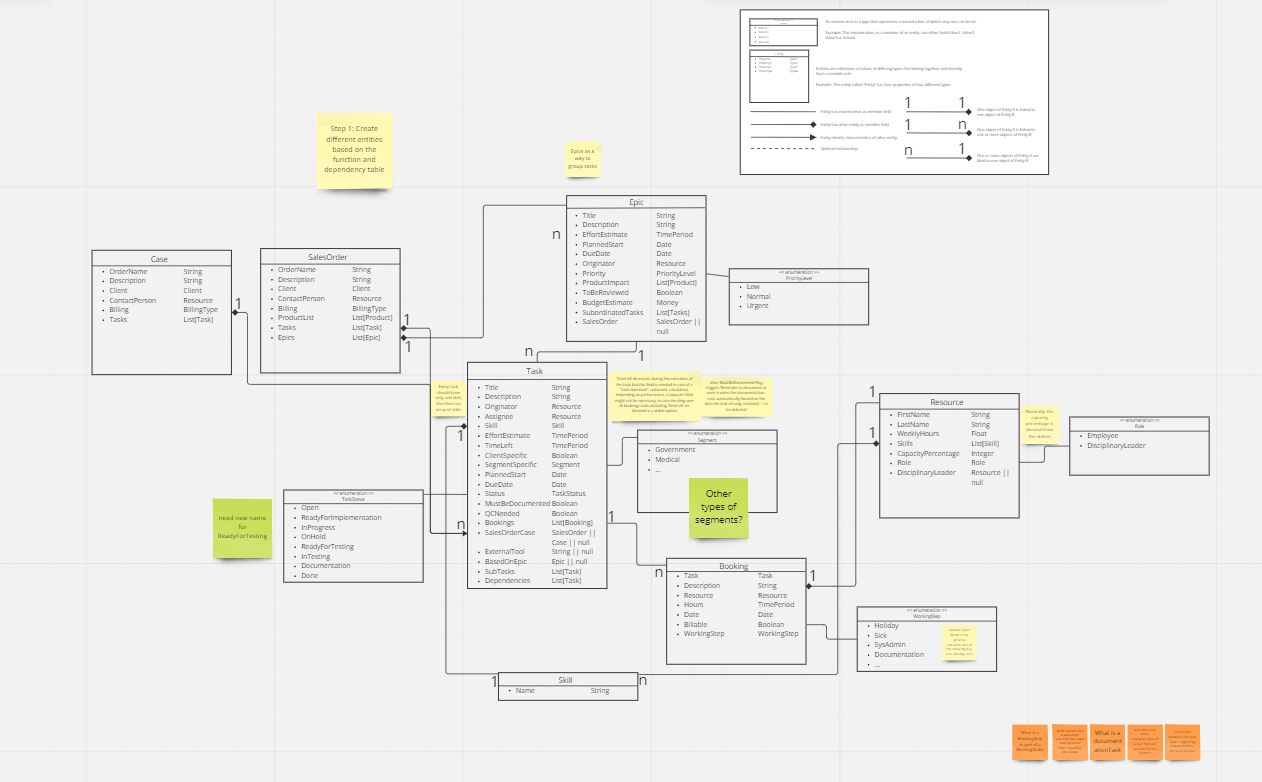
\includegraphics[width=0.75\textwidth]{img/miro_erschema.png}
    \caption{Finalisiertes ER-Schema, auf welchem das zukünftige System aufbauen soll.}
\end{figure}

Neben einer oberflächlichen Prozessplanung habe ich an diesem Tag auch begonnen, einzelne Teilprozesse dieser Planung in eine genauere Flowchart-Implementierung umzusetzen.

\subsubsection*{7. Februar - 9:00 bis 15:15 Uhr}
An diesem Arbeitstag habe ich die Teilprozessmodellierung fortgesetzt, wobei der Fokus mehr und mehr in die Detailplanung übergeht. Hieraus entstehen viele neue Fragen, die später mit dem Team abgeklärt werden müssen.

\subsubsection*{8. Februar - 10:00 bis 17:00 Uhr}
Auch an diesem Tag nahm die Detailplanung der Prozesse einen Teil ein. Jedoch bestand die zweite Hälfte des Arbeitstages daraus, ein präsentierbares Organigramm für eine spätere Präsentation des Systems zu erstellen. Dafür habe ich zu Beginn verschiedene Tools (Prezi, Canva, etc.) ausprobiert, da mir die Wahl des zu verwendenden Tools freigestellt wurde. Jedoch landete ich letztendlich bei Microsoft PowerPoint, da diese Applikation alle nötigen Werkzeuge und Vorlagen mitbringt, um optisch ansprechende Organigramme einer Organisation anzufertigen. 

Der Arbeitstag endete mit einem Teams-Call mit Carlos, bei dem ich Feedback zu meinem bestehenden Fortschritt bekommen habe. Dort habe ich erfahren, dass meine Ansätze seiner Meinung nach etwas zu komplex sind, worauf ich mir die Simplifizierung meines Modells als Ziel vorgenommen habe.

\subsubsection*{9. Februar - 8:45 bis 15:15 Uhr}
Der heutige Tag bestand darin, das Organigramm, mit welchem ich gestern begonnen habe, mit Fotos von den Mitarbeitern zu ergänzen, um das Gesamtkonzept ansprechender zu gestalten. Dazu habe ich einen Zugang zu dem unternehmensinternen Fotoarchiv erhalten.
Darauf folgend setzte ich das Feedback, welches ich am vorherigen Tag erhalten habe, in das Modell um.

Im Anschluss hatte ich ein persönliches Meeting mit meinem Betreuer, bei dem ich meine Fortschritte vorstellen und mögliche Fragen stellen konnte. Nach diesem Meeting lud uns mein Betreuer zum Mittagessen ein. Der Nachmittag endete für mich mit meinem ersten Meeting mit allen Mitarbeitern, die an dem Change-Prozess, dessen Kernsystem ich modellieren darf, beteiligt sind. Auch dort habe ich nochmals Feedback zu den Entitäten und Prozessen erhalten und durfte an der Gestaltung von verschiedenen Personas im Unternehmen, auf welche bei der Einführung des neuen Systems besonders geachtet werden muss, teilnehmen.

\subsubsection*{10. Februar - 10:00 bis 16:45 Uhr}
An diesem Tag habe ich mich ausschließlich mit der Implementierung des zuletzt gegebenen Feedbacks beschäftigt, da dies einige grundlegende Umstrukturierungen erforderte.

\subsubsection*{13. Februar - 8:00 bis 15:00 Uhr}
Der heutige Tag begann ebenfalls mit der Fortsetzung der Umsetzung des gegebenen Feedbacks. Im Anschluss recherchierte ich zu Microsoft Dynamics 365 Project Operations, da wir in dem Gruppenmeeting potenzielle Komplikationen, welche zwischen dem gewünschten und dem von Microsoft vorgegebenen System bestehen könnten, besprochen haben.

\subsubsection*{14. Februar - 8:45 bis 15:15 Uhr}
Um weitere mögliche logische Fehler in meinem Prozess- und Entitätenmodell zu finden, habe ich begonnen, den gesamten Prozess mit beispielhaften Daten zu simulieren. Hierbei wurde darauf geachtet, dass möglichst alle Teile der Flow-Diagramme ausgeführt werden, um Fehler in \enquote{seltenen Sondersituationen} zu entlarven.

\begin{figure}[h]
    \centering
    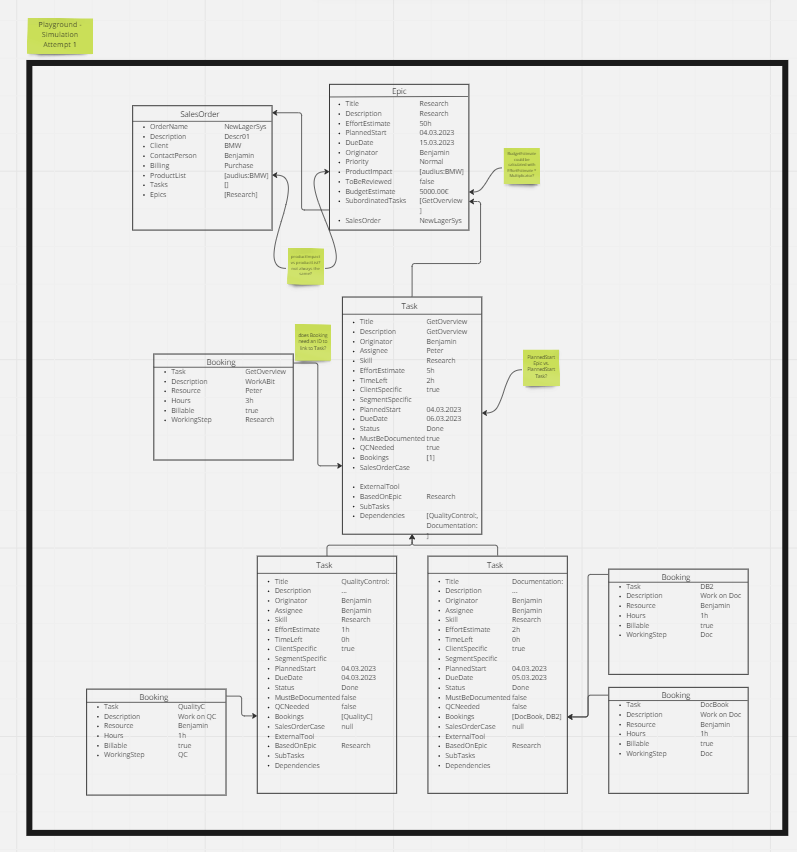
\includegraphics[width=0.75\textwidth]{img/miro_simulation.png}
    \caption{Entities nach der Simulation (CRUD-Operationen) durch verschiedene Subprozesse}
\end{figure}

Nachdem das gesamte Team zusammen zu Mittag gegessen hatte, filmten wir einen kurzen Imageclip, welcher für interne Zwecke bei einem jährlichen \enquote{Kickoff} gezeigt werden soll.

\subsubsection*{15. Februar - 9:15 bis 16:15 Uhr}
An diesem Tag beschäftigte ich mich zu Beginn mit dem Anpassen der Präsentation bzgl. dem Organigramm, da dieses noch etwas zu hierarchisch gewirkt hatte. Daher wählte ich eine holokratische Darstellungsform, um der de-facto flachen Organisationsstruktur gerecht zu werden. 

Im Anschluss nutzte ich meinen Zugang zu der unternehmensinternen Instanz von Microsoft Dynamics 365 Project Operations, um einen rudimentären digitalen Zwilling meiner bisherigen Praktikumstätigkeiten anzulegen. Diesen habe ich dann genutzt, um die Entitäten aus dem modellierten ER-Schema auf reale, bereits bestehende Entitäten in Project Operations umzulegen.

\subsubsection*{16. Februar - 8:45 bis 15:15 Uhr}
Heute beschäftigte ich mich primär erneut damit, das Prozessmodell zu simulieren, da ich bei der letzten Iteration einige Änderungen vorgenommen habe und daher einen \enquote{fehlerfreien Durchlauf} erzielen wollte.

\subsubsection*{17. Februar - 8:45 bis 16:15 Uhr}
Nachdem die Prozesse und Entitäten so weit abgeschlossen sind, begann nun die dokumentierte Fit/Gap-Analyse zwischen dem erstellen Framework und Microsoft Dynamics 365 Project Operations. Diese hat das Ziel, herauszufinden, welche Elemente des selbst gestalteten Prozesses in das Tool übernommen werden können, sowie Segmente, bei denen es potenziell Probleme geben könnte.

Um diese Herausforderung anzugehen, beschäftigte ich mich zu Beginn mit verschiedenen Ansätzen, wie Fit/Gap-Analysen im Business-Kontext normalerweise angegangen werden. Hierbei ist das Wissen, welches ich in der VL Betriebliche Standardsoftware bzgl. Fit/Gap-Analysen gewonnen habe, von Nutzen. Im Anschluss erstellte ich, basierend auf meinen gestalteten Prozessen, eine Liste an beschriebenen Anforderungen, auf welche Project Operations anschließend geprüft wird, um Fits und Gaps auszumachen.

\subsubsection*{20. Februar - 8:45 bis 15:15 Uhr}
An dem heutigen Tag habe ich mich primär damit beschäftigt, Microsoft Dynanmics Project Operations auf das zuletzt erstellte Anforderungsprofil zu prüfen. Im Fokus standen dabei Solutions, welche das Erstellen von benutzerdefinierten Entitäten und Feldern ermöglichen.

\begin{figure}[h]
    \centering
    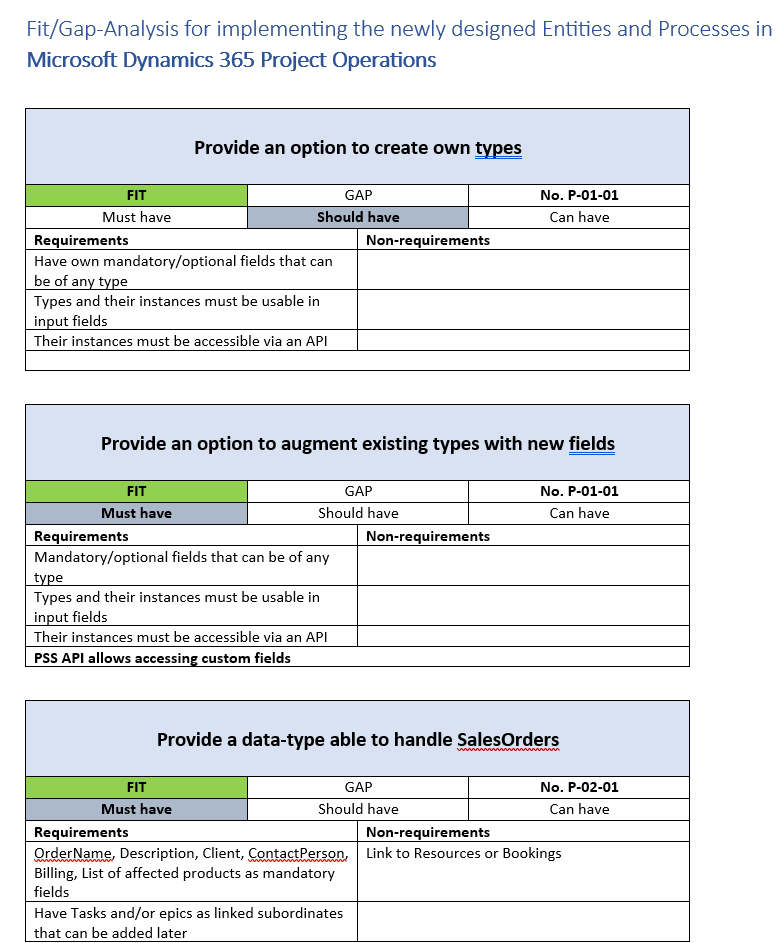
\includegraphics[width=0.75\textwidth]{img/fit_gap.png}
    \caption{Auszug aus der FIT/GAP-Analyse für Microsoft Project Operations mitsamt Anforderungsprofil}
\end{figure}

\subsubsection*{21. Februar - 8:00 bis 15:15 Uhr}
Nachdem ich mir eine eigene virtuelle Umgebung mitsamt Microsoft Dataverse Datenbank angelegt habe, konnte ich mich Microsoft PowerApps widmen. In diesem Tool ist es möglich, Felder und Entitäten benutzerdefiniert zu bearbeiten, womit ich versucht habe, Dynamics 365 Project Operations auf die Anforderungen des Entity-Modells zu trimmen.

\subsubsection*{22. Februar - 8:45 bis 15:15 Uhr}
An diesem Tag versuchte ich weiter, das bestehende Project Operations an den gestalteten Prozess anzugleichen. Hierbei stoß ich auf einige Architekturprobleme, welche in dem nächsten Meeting mit den verantwortlichen Kollegen besprochen werden müssen.

\subsubsection*{23. Februar - 8:45 bis 15:30 Uhr}
Heute setzte ich mich mit den Möglichkeiten auseinander, Dynamics 365 Dashboards zu erstellen. Diese sollen den Mitarbeitern direkt und ohne Submenüs ihre verbleibende Kapazität und die zugewiesenen Aufgaben darstellen. Der Tag endete mit einem Meeting mit allen Beteiligten, bei welchem wir die aufgetretenen Probleme besprochen und gemeinsam einen neuen Plan für das weitere Vorgehen entwickelt haben.

\subsubsection*{24. Februar - 8:45 bis 15:15 Uhr}
Heute erweiterte ich die erstellten Dashboards und recherchierte bzgl. eines externen Tools, mit welchem ER-Diagramme aus Microsoft Dataverse Datenbanken erstellt werden können. Dies wird in Zukunft nützlich sein, wenn es darum geht, herauszufinden, welche Komponenten von Project Operations für das Projekt nutzbar sind und welche Komponenten evtl. substituiert werden müssen.

\subsubsection*{27. Februar - 8:45 bis 15:15 Uhr}
An diesem Tag setzte ich mich mit PowerBI-Dashboards, der zugehörigen Skriptsprache DAX und dem bestehenden Datenmodell auseinander, um ein optisch-ansprechendes Dashboard zu erzeugen, welches die  Arbeitsstunden, die ein Mitarbeiter diese Woche bereits alloziert hat, anzeigt.

\subsubsection*{28. Februar - 8:45 bis 15:15 Uhr}
Der heutige Tag setzte sich aus dem Erstellen eines Projektmanager-Dashboards, auf dem die Aktivitäten des gesamten Teams dargestellt werden, sowie aus dem Überarbeiten des persönlichen Dashboards zusammen.

\subsection{März}
\subsubsection*{1. März - 9:00 bis 15:45 Uhr}
Nachdem die erstellten Dashboards eine sehr schlechte Performance aufgewiesen hatten, beschäftigte ich mich heute damit, die Berechnungen mit PowerQuery und der zugehörigen relationalen Sprache M umzusetzen, was letztendlich gelungen ist. Das Mitarbeiterdashboard und das PM-Dashboard sind somit fertiggestellt, womit die beiden zugehörigen Anforderungen als FIT markiert werden können.

\subsubsection*{2. März - 8:45 bis 15:15 Uhr}
Heute finalisierte ich die Dashboards und recherchierte bzgl. dem Exportieren meiner bisherigen Arbeit, damit diese dann in der Umgebung, auf welcher Project Operations final laufen soll, importiert werden kann. Nachdem dies erledigt ist, kann ich mich mit der Prozessimplementierung beschäftigen.

\subsubsection*{3. März - 8:45 bis 15:15 Uhr}
An diesem Tag setzte ich mich mit den Möglichkeiten bzgl. der Implementierung der Background-Logik auseinander. Dabei ist einerseits der Zugang mittels PowerAutomate Flows möglich, jedoch auch die WebAPI, welche - auf dem REST-Konzept aufbauend - CRUD-Operationen zulässt. Hierbei läge der Vorteil darin, dass keine Kosten pro Flow, wie in PowerAutomate, anfallen würden.

\subsubsection*{6. März - 8:45 bis 15:45 Uhr}
Der Fokus des heutigen Tages lag auf der Implementierung von Validierungsprozessen in JavaScript. Damit können diese als Teil der Inputformulare in PowerApps ausgeführt werden, was eine Inputvalidierung direkt bei der Eingabe und nicht erst nach der Speicherung möglicherweise fehlerhafter Datensätze ermöglicht. Darüber hinaus habe ich die Dashboards so ergänzt, dass diese auch dann sinnvolle Inhalte anzeigen, wenn diese Woche noch gar keine Buchungen oder Task-Zuweisungen stattgefunden haben.

\subsubsection*{7. März - 8:45 bis 15:15 Uhr}
Heute begann ich mit dem Umsetzen des Status Flags, welcher für jede Projektaufgabe gesetzt ist und welcher überwiegend automatisch gemanaged werden soll. Die automatischen Prüfungen wurden erneut in JavaScript umgesetzt, wobei die erstaunlich gute Performance bei Dataverse Datenbankabfragen positiv auffiel. Somit lassen sich die Möglichkeiten für den Nutzer, Felder auf nicht zulässige Art und Weise zu verändern, minimieren.

\subsubsection*{8. März - 8:45 bis 15:15 Uhr}
Dieser Tag war überwiegend von Recherchen bzgl. der Ausführung von Microsoft Dataverse Actons über die JavaScript API geprägt. Hierbei fiel auf, dass die Dokumentation, welche Microsoft für derartige Anwendungsfälle zur Verfügung stellt, tendenziell eher unzureichend sind. Dies könnte damit zusammenhängen, dass die gleichen Aktionen auch über das kostenpflichtige PowerAutomate mit Dataverse Flows erreicht werden kann.

\subsubsection*{9. März - 8:45 bis 15:15}
Das Ziel des heutigen Tages war es, Tasks über die JavaScript API erstellen zu können, sowie diese in eine hierarchische Zuordnung zu bringen. Dieses Thema stellte sich als überaus fordernd heraus, da die Dokumentation seitens Microsoft nicht für die Durchführung mit JavaScript verfügbar ist. Jedoch endete der Tag mit dem erfolgreichen Anlegen von Tasks über JS.

\subsubsection*{10. März - 8:15 bis 14:30}
Nach dem gestrigen Erfolg habe ich heute die komplette Logik der automatisch generierten Dependency-Tasks in JavaScript umgesetzt. Nun muss sich der Anwender des Systems nicht mehr selbst darum kümmern, dass notwendige Tasks zur Dokumentation und für das Qualitätsmanagement getaner Arbeit angelegt werden.

\subsection{April}

\subsection{Mai}
